\part{Automatique}
\section{Introduction}
\underline{Objet du cours} : Analyser et faire une synthèse d'un système physique (soumis aux lois de la dynamique, et suivant des équations).\\
En automatique, \textit{un système} (S) est caractérisé par deux grandeurs :
\begin{itemize}
	\item Les entrées, qui s'appliquent à S et agissent sur son état. Il y en a de 2 types : 
		\begin{itemize}
			\item Sur lesquels on peut agir (les forces)
			\item Sur lesquels on ne peut pas agir (frottements, perturbations...)
		\end{itemize}
	\item Les sorties, qui sont des grandeurs élaborées par S sous l'action des entrées.
\end{itemize}

\bigskip
Le but est de déterminer les entrées qu'il faut pour avoir les résultats désirés. 

\Exemp{}{Pour un avion, quelles entrées (vitesse, altitude...) faut-il appliquer pour suivre une trajectoire donnée ?}

On identifie spécialement deux classes :
\begin{itemize}
	\item Les systèmes linéaires ou non linéaires
	\item Les systèmes variants ou invariants (sous-entendu : dans le temps)
\end{itemize}

\bigskip
\Def{}{Soit S un système. S est dit linéaire si l'application entrée/sortie est linéaire, ie :
	\begin{tikzpicture}
		\draw [->] (0,2) -- (1,2) ;
		\draw (0,2) node[left] {$u(t)$} ;
		\draw (2,2) circle (1);
		\draw (2,2) node{$S$};
		\draw [->] (3,2) -- (4,2);
		\draw (4,2) node[right] {$y(t)$};
		\draw [->] (0,-2) -- (1,-2);
		\draw (0,-2) node[left] {$v(t)$} ;
		\draw (2,-2) circle (1);
		\draw (2,-2) node{$S$};
		\draw [->] (3,-2) -- (4,-2);
		\draw (4,-2) node[right] {$z(t)$};
		\draw (6,0) node{$\Rightarrow$} ;
		\draw [->] (10,0) -- (11,0) ;
		\draw (10,0) node[left] {$\lambda u(t)+\mu v(t)$} ;
		\draw (12,0) circle (1);
		\draw (12,0) node{$S$};
		\draw [->] (13,0) -- (14,0);
		\draw (14,0) node[right] {$\lambda y(t)+\mu z(t)$};
	\end{tikzpicture}

	S est dit invariant si :\\
	y(t) est la sortie (ou la réponse) du système S par l'action de l'entrée u(t), pour $t\in[t_0,T[$.
	\begin{tikzpicture}
		\draw [->] (0,0) -- (1,0) ;
		\draw (0,0) node[left] {$u(t)$} ;
		\draw (2,0) circle (1);
		\draw (2,0) node{$S$};
		\draw [->] (3,0) -- (4,0);
		\draw (4,0) node[right] {$y(t)$};
		\draw (7,0) node{$\Rightarrow$} ;
		\draw [->] (10,0) -- (11,0) ;
		\draw (10,0) node[left] {$u_{\tau}(t)$} ;
		\draw (12,0) circle (1);
		\draw (12,0) node{$S$};
		\draw [->] (13,0) -- (14,0);
		\draw (14,0) node[right] {$y_{\tau}(t)$};
	\end{tikzpicture}
	Avec $\tau>0$ et $u_{\tau}:t\mapsto u(t-\tau)$
}

\Exemp{}{Soit S donné par :
\begin{itemize}
	\item $y'(t)=u(t)$ : linéaire invariant
	\item $y^2(t)+y''(t)=u(t)$ : non linéaire invariant
	\item $ty'(t)+ky''(t)=u(t)+u'(t)$ : linéaire variant
\end{itemize}
}

Il y a deux types d'études :
\begin{itemize}
	\item l'étude externe : elle n'est basée que sur les entrées et les sorties
	\item l'étude interne : elle utilise l'état de S chaque instant t
\end{itemize}

\underline{Le but du cours sera donc d'étudier :}
\begin{itemize}
	\item La contrôlabilité : aller d'un point initial à un point final
	\item L'observabilité : mesurer entrées et sorties pour trouver l'état $x(t_0)$ de S
	\item La stabilité : le système est-il stable ? Est-il possible de le stabiliser ?
\end{itemize}

\section{Représentation d'état}
Soit S un système :\\
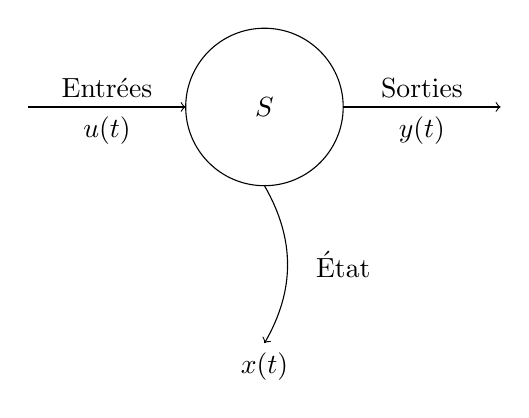
\begin{tikzpicture}
	\draw [->] (0,0) -- (2,0) ;
	\draw (1,0) node[above] {Entrées} ;
	\draw (1,0) node[below] {$u(t)$} ;
	\draw (3,0) circle (1);
	\draw (3,0) node{$S$};
	\draw [->] (4,0) -- (6,0);
	\draw (5,0) node[above] {Sorties} ;
	\draw (5,0) node[below] {$y(t)$};
	\draw [->] (3,-1) to[bend left] (3,-3);
	\draw (4,-2) node{État};
	\draw (3,-3) node[below]{$x(t)$};
\end{tikzpicture}

\begin{itemize}
	\item $u(t)$ : les entrées (commandes ou contrôles) avec m entrées : $u(t)\in\mathbb{R}^m$
	\item $y(t)$ : les sorties, avec p sorties : $y(t)\in\mathbb{R}^p$
	\item $x(t)$ : vecteur d'état : n variables indépendantes pour définir l'état de S à chaque instant $t\in[t_0,T[$. 
\end{itemize}

L'équation d'état est de la forme : 
\[\dot{x}(t)=f(x(t),u(t))\]
L'équation de sortie :
\[y(t)=h(x(t))\]

\Exemp{}{ \[\dot{x}(t)=2x(t)+u(t),\ x(t)\in\mathbb{R}, u(t)\in\mathbb{R}\] 
	\[y(t)=5x(t),\ y(t)\in\mathbb{R}\]

m=n=p=1

\[\dot{x}(t)=\binom{x_1(t)+u_1(t)x_2^2(t)}{x_1(t)x_2(t)+u_2^2(t)}\]
\[y(t)=e^{x_1(t)x_2(t)}\]
}

\underline{\textit{Remarque :}} Si $u(t)=cst=k$, l'équation d'état est de la forme $\dot{x}(t)=f(x(t),k)$.\\
Si $u(t)=\alpha x(t)$ une fonction de l'état, alors $\dot{x}(t)=f(x(t),\alpha x(t)$. On obtient donc un système dynamique de la forme :
\[\dot{z}(t)=F(z(t))\]

\bigskip
Pour une entrée donnée $u:[t_0,T]\to\mathbb{R}^m$ et $x(t_0)$ une condition initiale, on note $x_u(t,x(t_0))$ la solution à l'instant t de $\dot{x}(t)=f(x(t),u(t)$ de condition initale $x(t_0)$.\\
Pour simplifier, on marque en général 
\[x(t)=x_u(t,x(t_0))\]

\bigskip
\Def{}{\begin{itemize}
\item Un état z est dit accessible à partir d'un état inital $x(t_0)$ sous l'entrée $u:[t_0,T]\to\mathbb{R}^m$ si $z=x_u(t,x(t_0))$ pour un certain $t\in[t_0,T]$.
\item On appelle \textit{ensemble d'accessibilité à partir de $x(t_0)$ sous l'action de $u$} l'ensemble :
\[\mathcal{A}_u(x(t_0),u)=\{x_u(t,x(t_0)),\ t\in[t_0,T]\]
\item S est dit contrôlable à partir de $x(t_0)$ sur l'espace d'état $E\subset \mathbb{R}^n$ si :
\[\forall z\in E;\ \exists u:[t_0,T]\ |\ z=x_u(t,x(t_0))\]
\item S est dit complètement contrôlable sur E si $\forall z_1,z_2\in E$, il existe $u:[t_0,T]\to\mathbb{R}^m$ qui permet de transformer S de l'état $z_1$ à $z_2$, c'est-à-dire :
\[\exists t\in[t_0,T];\ z_2=x_u(t,z_1)\]
\end{itemize}}

\Exemp{}{$S:\dot{x}(t)=(x(t)+u(t))^2$, avec $x(t_0)$ donné, $x(t)\in E\subset \mathbb{R}$ et $u(t)\in\mathbb{R}$.\\
S est-il complètement contrôlable sur $\mathbb{R}$ ?

\bigskip
$\dot{x}(t)\geq 0$, donc $x(t)$ ne peut que croître depuis $x(t_0)$.\\
Par exemple, l'état $z_2=x(t_0)-1$ n'est jamais accessible à partir de $x(t_0),\ \forall u$. S n'est donc pas complètement controlable.}

\Rap{}{\begin{itemize}
\item La solution à l'équation $\dot{x}(t)=Ax(t)+Bu(t)$, avec $x(t)\in\mathbb{R}^n$, $u(t)\in\mathbb{R}^m$, $A$ matrice $(n,n)$ et $B$ matrice $(n,m)$, toutes deux constantes, est :
\[x(t)=e^{A(t-t_0)}x(t_0)+e^{At}\int_{t_0}^t e^{-As}Bu(s)ds\]
\item Pour calculer $e^A$ :
	\begin{itemize}
		\item[$\bullet$] On utilise la définition : \[e^A=\sum_{k=0}^{+\infty} \frac{A^k}{k!}\]
		\item[$\bullet$] Si $MN=NM$, alors $e^{M+N}=e^Me^N$
		\item[$\bullet$] Si $A$ est diagonalisable, alors $A=PDP^{-1}$ et donc $e^A=Pe^DP^{-1}$
		\item[$\bullet$] On utilise la tranformée de Laplace :
			\[\mathcal{L} : f \mapsto \mathcal{L}(f)(s)=\int_0^{+\infty} e^-st f(t) dt\]
	\end{itemize}

\item Propriétés de la transformée de Laplace :
	\begin{itemize}
		\item[$\bullet$] $\mathcal{L}$ est linéaire.
		\item[$\bullet$] Elle permet de passer d'une équation différentielle à une équation algébrique :
			\[\mathcal{L}(f')(s)=s\mathcal{L}(f)(s)-f(0)\]
		\item[$\bullet$] Si $f(0)=...=f^{(n)}(0)=0$ :
			\[\mathcal{L}(f^{(n)})(s)=s^n\mathcal{L}(f)(s)\]
		\item[$\bullet$] À savoir :
			\[\mathcal{L}(\cos(\omega t)) = \frac{s}{s^2+\omega^2}\]
			\[\mathcal{L}(\sin(\omega t)) = \frac{\omega}{s^2+\omega^2}\]
			\[\mathcal{L}(e^{kt}) = \frac{1}{s-k}\]
	\end{itemize}
\end{itemize}}

\subsection{Fonction (ou matrice) de transfert}

\Def{}{La fonction (ou matrice) de transfert d'un système $S$ est une relation Entrée / Sortie donné en variable de Laplace :
	\[Y(s)=G(s)U(s) \Leftrightarrow\]
\centering 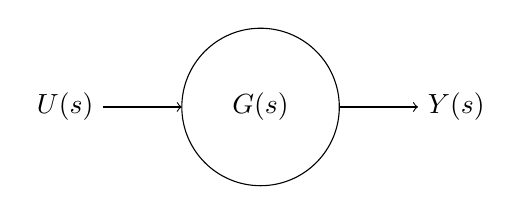
\begin{tikzpicture}
		\draw [->] (0,0) -- (1,0) ;
		\draw (0,0) node[left] {$U(s)$} ;
		\draw (2,0) circle (1);
		\draw (2,0) node{$G(s)$};
		\draw [->] (3,0) -- (4,0);
		\draw (4,0) node[right] {$Y(s)$};
	\end{tikzpicture}
}

\Prop{}{Si $S:y^{(n)}(t)+a_{n-1}y^{(n-1)}(t)+...+A_0y(t)=u(t)$, avec $y(t)\in\mathbb{R}$ et $u(t)\in\mathbb{R}$, $a_i$ constante réelle, $i=0,...,n-1$.\\
On suppose que $y^{(n-1)}(0)=...=y(0)=0$. Alors :
\[G(s)=\frac{1}{s^n+...+a_1s+a_0}\]
Les pôles de $G(s)$ sont les zéros du dénomniateur.}

\Exemp{}{$S$ est un système donné par sa fonction de transfert : \[G(s)=\frac{1}{s^2-1}\] avec $y(0)=y'(0)=0$
\begin{eqnarray*}
Y(s)=G(s)U(s)\\
s^2Y(s)-Y(s)=U(s)\\
y''(t)-y(t)=u(t)
\end{eqnarray*}}

\subsection{Observabilité - Observateur}
\Def{Observable}{Soit S un système d'entrée $u(y)$ et de sortie $y(t)$, $t\in[t_0,T]$.\\
S est dit observable à l'instant $t_0$ si connaissant toutes les entrées et les sorties sur $[t_0,T]$, on peut déterminer l'état initial $x(t_0)$ de façon unique.}

\Def{}{Un observateur pour $S$ est un système auxiliaire qui a pour entrée $u(t)$ et $y(t)$ et pour sortie $\hat{x}(t)$ un état estimé de $S$.}

\underline{Remarque :} L'idéal est que $e(t)=x(t)-\hat{x}(t)$ (erreur entre l'état réel et l'état estimé) tende vers 0.\\
\begin{center}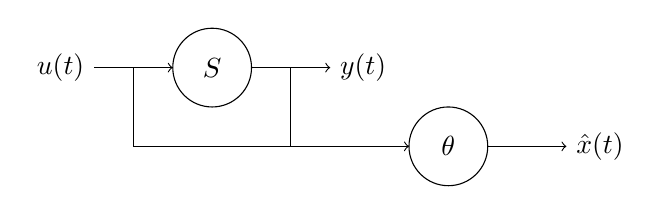
\begin{tikzpicture}
	%Système 1
	\draw [->] (0,0) -- (1,0) ;
	\draw (0,0) node[left] {$u(t)$} ;
	\draw (1.5,0) circle (0.5);
	\draw (1.5,0) node{$S$};
	\draw [->] (2,0) -- (3,0);
	\draw (3,0) node[right] {$y(t)$};
	%Flèches vers système 2
	\draw [->] (0.5,0)--(0.5,-1)--(4,-1);
	\draw (2.5,0)--(2.5,-1);
	%Système 2
	\draw (4.5,-1) circle(0.5);
	\draw (4.5,-1) node{$\theta$};
	\draw [->] (5,-1)--(6,-1);
	\draw (6,-1) node[right] {$\hat{x}(t)$};
\end{tikzpicture}\end{center}

\subsection{Points d'équilibre - Stabilité}
\Def{Stabilité}{Soit $S$ donné par l'équation d'état \[\dot{x}(t)=f(x(t),u(t))\]
L'état $x(t_0)$ est stable si, $\forall x_1$, état proche de $x_0$, la trajectoire $x_u(t,x_1)$ reste proche de $x_u(t,x_0)$ $\forall t$.}

\Def{Point d'équilibre}{On dit que $(x_0,u_0)$ est point d'équilibre si $f(x_0,u_0)=0$.}

